\documentclass[11pt]{article}

\usepackage[margin=0.85in]{geometry}
\usepackage{amsmath, amssymb}
\usepackage{graphicx}
\usepackage{booktabs}
\usepackage{tikz}
\usetikzlibrary{positioning}
\usepackage{hyperref}
\usepackage{natbib}
\setlength{\bibsep}{0pt plus 0.3ex}
\emergencystretch=10em

\title{Auditing the 3rd-Place Solution to the Jigsaw Unintended Bias in Toxicity Classification Competition}
\author{Ian Tang and Nick Chen \\ DS-UA 202: Responsible Data Science, Spring 2026 \\ Group 21}
\date{\today}

\begin{document}
\maketitle

% rubric §1: ADS overview, stated goals, trade-offs between goals
\section{Introduction}

Toxicity classifiers are decision-support systems whose prediction errors land on real people: a wrongful flag silences a person's voice in a public conversation, and a missed slur leaves a targeted reader exposed to the harm the platform was meant to absorb. The audit's central question is whose voice and whose dignity the deployed model treats equivalently across identity lines. This report audits the third-place finishing solution to the 2019 Jigsaw \emph{Unintended Bias in Toxicity Classification} Kaggle competition, a publicly available toxicity-classification ensemble built by sakami0000 \citep{sakami2019jigsaw}. The 2019 competition was itself the followup to Jigsaw's 2018 \emph{Toxic Comment Classification Challenge}: the Subgroup/BPSN/BNSP power-mean scoring rule we critique here was Jigsaw's deliberate response to the identity--toxicity correlations the 2018 plain-AUC scoring rewarded \citep{borkan2019nuanced}. The metric is therefore itself a corrective-design artifact carrying its own normative commitments; the audit pairs system analysis (\S5.1--\S5.3) with metric-design analysis (\S5.4) as co-equal objects, on the conviction that a model passing a normatively unjustifiable metric has not passed an audit. We audit a faithful 2-of-5-component recreation of the original five-component F.H.S.D.Y.\ ensemble (\texttt{bert-large-uncased} + LSTM--GRU under Optuna-tuned blend weights; \S4.1 details the scoping commitments). The dataset is the Civil Comments corpus, released by Jigsaw alongside the 2019 competition.

The audit takes a normative spine. The system implicitly enacts a particular theory of fairness through the metric it was trained against, the threshold at which it is deployed, the identity columns that metric evaluates, and the rater procedure that produced its training labels. Each is a value-laden choice the developers and the competition designers left implicit. Our task is to name the choices, test how well the implementation realizes the fairness ideals they encode, and surface the trade-offs the developers could not have avoided. With base rates that differ across identity subgroups, the Chouldechova impossibility result \citep{chouldechova2017fair} guarantees that no single fairness metric is neutral; the choice of which condition to privilege is therefore a stakeholder choice. Every numerical result reported in \S5 is anchored to one of these normative claims.

\section{Background}

The 2019 Kaggle \emph{Unintended Bias in Toxicity Classification} competition was paired with the Civil Comments corpus \citep{borkan2019nuanced}, $\sim$1.8M crowd-rated comments released by Jigsaw with toxicity and identity annotations (\S3.1). Participants were asked to maximize toxicity-prediction rank quality while minimizing unintended bias against identity subgroups whose mention correlates with toxic content. The competition encoded the trade-off as a bias-aware score combining Overall AUC (weight $0.25$) with a generalized power mean ($p = -5$) over per-identity bias AUCs (weight $0.75$), evaluated on nine of the twenty-four identity columns the dataset annotates. The $25/75$ weighting, the exponent $p = -5$, and the nine-of-twenty-four cutoff each encode a normative claim \S5.4 unpacks. We audit the recreated BERT-large + LSTM-GRU ensemble of \citet{sakami2019jigsaw}; the recreation reproduces two of the five original components (\S4.1).

% rubric §2: input feature profiling, output interpretation
\section{Input and Output}

\subsection{Civil Comments and identity-subgroup coverage}

The audit runs on the private test set of the Civil Comments corpus ($n = 97{,}320$). Civil Comments operated as a third-party comment-hosting platform for English-language news sites between 2015 and 2017; the public release contains approximately $1.8$M comments collected when the platform shut down.

Each comment was annotated along two tracks. The toxicity track records a primary \texttt{toxicity} label and six subtype labels (\texttt{severe\_toxicity}, \texttt{obscene}, \texttt{identity\_attack}, \texttt{insult}, \texttt{threat}, \texttt{sexual\_explicit}), each as the fraction of raters who applied the label. The identity track records twenty-four attributes spanning gender (4), sexual orientation (4), religion (7), race/ethnicity (5), and disability (4), each as the fraction of identity-annotators who marked the identity as referenced. Following Civil Comments convention, an identity is treated as ``mentioned'' when its column value is at least~$0.5$.

At threshold~$0.5$, the nine identities the bias-aware metric evaluates---\texttt{male}, \texttt{female}, \texttt{homosexual\_gay\_or\_lesbian}, \texttt{christian}, \texttt{jewish}, \texttt{muslim}, \texttt{black}, \texttt{white}, \texttt{psychiatric\_or\_mental\_illness}---together account for $11{,}003$ mentions; the fifteen excluded identities (\texttt{transgender}, \texttt{heterosexual}, \texttt{bisexual}, \texttt{asian}, \texttt{latino}, \texttt{hindu}, \texttt{buddhist}, \texttt{atheist}, the four \texttt{other\_*} category-residual columns, and every disability category other than \texttt{psychiatric\_or\_mental\_illness}) account for only $807$ in aggregate. All evaluated subgroups have $n \geq 238$ at this threshold; all excluded have $n \leq 217$. The selection appears sample-size driven---revisited in \S5.4. Per-group base rates among evaluated identities, as observed on the private test set, span $[0.0996, 0.3233]$ (\texttt{christian} to \texttt{black}); this range is binding for \S5.2's impossibility result.

\subsection{Output: toxicity score and thresholding}

The system produces seven floating-point outputs per comment, each in $[0, 1]$: a primary toxicity score $\hat{Y}$ and six subtype scores. Each score is trained to approximate the fraction of Civil Comments raters who applied the corresponding label. The competition metric and our \S5.1 accuracy analysis treat $\hat{Y}$ as a continuous score and use AUC-style measures. Our \S5.2 fairness analysis thresholds $\hat{Y}$ at $s_{HR} = 0.5$ to recover a binary moderation decision and report the resulting confusion-matrix metrics. We adopt $0.5$ as a deliberately conventional choice---the default a deployed moderation pipeline would inherit from any binary classifier---so a reader who prefers a different operating point can substitute it without re-running the model.

\subsection{The toxicity label as a measurement choice}

The toxicity label we audit against is itself the product of a measurement choice: it is the fraction of crowd-worker raters who applied the ``toxic'' label to a given comment. This formulation embeds three commitments that downstream fairness analysis inherits. First, it treats toxicity as an aggregable property of the text rather than a property of the rater--text dyad: a label value of $0.4$ does not distinguish ``a coherent minority of raters found this toxic'' from ``most raters disagreed about whether it was toxic at all.'' Second, training and evaluation both binarize the score around $0.5$, so if rater demographics under-represent any identity, that identity's rater consensus on what counts as toxic is structurally under-counted at the binarization step. Third, the rater pool is not demographically balanced to the populations the labels are \emph{about}. The audit that follows respects the label as given, but every fairness gap we report should be read modulo this upstream measurement choice---a different rater pool or a different aggregation rule could move some of the gaps materially.

% rubric §3: pre-processing, implementation, validation
\section{Implementation and Validation}

\subsection{Recreation scope and deviations from the original}

The original third-place solution was an F.H.S.D.Y.\ five-component ensemble combining several transformer- and recurrent-architecture variants together with fine-tuned GPT-2 language-model component(s). Recreating the full ensemble was infeasible within this project's compute budget; we therefore reproduced two of its components---\texttt{bert-large-uncased} fine-tuned for the competition's seven-way multi-task head, and a five-fold-averaged LSTM--GRU model with the same multi-task head structure---and combined them with Optuna-tuned blend weights. The fairness implication of this scoping is non-trivial. An ensemble whose structural diversity is reduced may encode a single component's inductive bias more sharply than the original; conversely, biases that the original ensemble averaged out across components may surface more visibly here. We return to this in \S5.3 (BERT vs.\ LSTM bias profiles) and \S6.4.

\subsection{Architecture: BERT-large-uncased + LSTM-GRU multi-task ensemble}

\texttt{bert-large-uncased} is the standard 24-layer, 1024-hidden, 16-attention-head transformer with $\sim$340M parameters; the recreation feeds its pooled output to seven linear heads (one toxicity head plus six subtype heads) and fine-tunes them jointly. The LSTM--GRU component is a recurrent sequence model with the same seven-head output structure, trained as a five-fold cross-validation ensemble whose per-fold scores are averaged at inference. Both models inherit Civil Comments' tokenization and preprocessing as distributed by Jigsaw, with no project-specific cleaning beyond what the original recipe specifies. The two models are trained independently; only their per-comment scores are combined at inference time.

\subsection{Validation: Optuna blend and competition-format reproduction}

The blended ensemble's per-comment toxicity score is the Optuna-tuned weighted mean of the BERT and LSTM scores. The optimizer returned blend weights of $(\,\text{BERT}: 0.993,\; \text{LSTM}: 0.007\,)$ on the validation fold, meaning that under the competition's bias-aware loss the LSTM contributes near-negligibly when BERT is available. We retain the LSTM in the audit nonetheless, because its standalone bias profile differs from BERT's in ways that are analytically informative even when its blend weight is small (\S5.3).

On the private test set ($n = 97{,}320$), the recreated ensemble reproduces the competition's bias-aware score at~$0.94464$, with component AUCs of $0.97368$ (Overall), $0.90183$ (mean Subgroup), $0.94762$ (mean BPSN), and $0.95544$ (mean BNSP). The original third-place private-leaderboard score was $0.94683$; the gap of $\sim 0.002$ is small enough that subsequent fairness gaps can be read against a faithful reproduction of competition-format performance, while large enough that we caveat against treating the recreation as a proxy for the original five-component ensemble's full bias profile (\S4.1, \S6.5 (i)). Operationally, ensemble predictions are within $\sim 1\%$ of BERT-alone scores; the LSTM enters the audit primarily as a counterfactual diagnostic for component-level bias divergence. Hyperparameters, seeds, and counterfactual templates are documented in \texttt{jigsaw\_audit\_analysis.ipynb} (cells 015, 020, 039).

% rubric §4: (a) accuracy, (b) fairness, (c) additional methods
\section{Outcomes}

\subsection{Discriminative parity across subpopulations}

Per-identity AUC disaggregation operationalizes a discriminative-parity reading of group fairness: a system is fair if its rank-ordering of toxic from non-toxic comments is equally informative across identity subgroups. The stakeholder this metric protects is the identity-group member harmed when the model's score function works less well for their group than for others, regardless of the direction the error tends. Following \citet{borkan2019nuanced}, we report three AUC variants per subgroup: \emph{Subgroup AUC} (separability of toxic from non-toxic \emph{within} the subgroup); \emph{BPSN AUC}, in which the positive class is toxic comments not mentioning the identity and the negative class is non-toxic comments mentioning the identity (a low BPSN flags over-flagging of benign mentions); and \emph{BNSP AUC}, in which the positive class is toxic comments mentioning the identity and the negative class is non-toxic background (a low BNSP flags under-flagging of toxicity targeting the group).

\begin{table}[h]
\centering
\small
\begin{tabular}{lrrrr}
\toprule
Identity & $n$ & Subgroup AUC & BPSN AUC & BNSP AUC \\
\midrule
male                          & 2112 & 0.9367 & 0.9621 & 0.9592 \\
female                        & 2602 & 0.9418 & 0.9722 & 0.9515 \\
homosexual gay or lesbian     &  538 & 0.8541 & 0.9298 & 0.9504 \\
christian                     & 2109 & 0.9475 & 0.9761 & 0.9471 \\
jewish                        &  411 & 0.9098 & 0.9541 & 0.9518 \\
muslim                        & 1054 & 0.8723 & 0.9424 & 0.9489 \\
black                         &  761 & 0.8670 & 0.9258 & 0.9573 \\
white                         & 1178 & 0.8738 & 0.9243 & 0.9593 \\
psychiatric or mental illness &  238 & 0.9560 & 0.9514 & 0.9753 \\
\midrule
\textit{power-mean ($p{=}{-}5$) across the 9}    &      & 0.9018 & 0.9476 & 0.9554 \\
\bottomrule
\end{tabular}
\caption{Per-identity bias AUCs on the private test set ($n = 97{,}320$). Identity counts use the $0.5$ mention-threshold convention. Means agree with the competition-format header reported in \texttt{cell029}.}
\label{tab:bias-aucs}
\end{table}

\begin{figure}[ht]
\centering
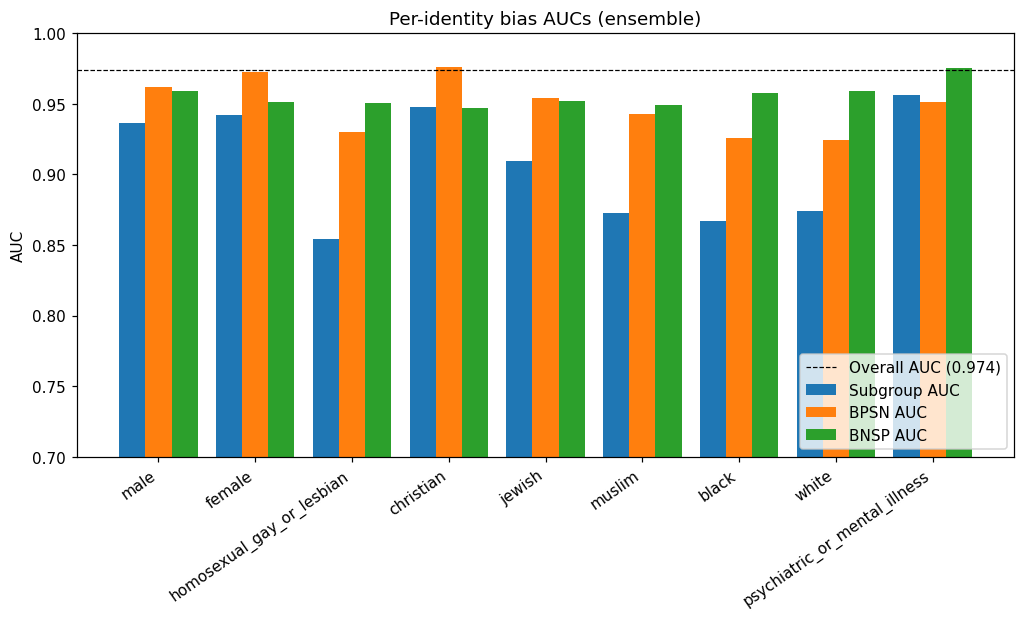
\includegraphics[width=0.85\linewidth]{inference_outputs/cell034_markdown-a-grouped-bar-chart-of-the-3-bias-aucs-per-identity_out00.png}
\caption{Subgroup, BPSN, and BNSP AUCs per evaluated identity (Table~\ref{tab:bias-aucs}). Low BPSN on \texttt{white}, \texttt{black}, and \texttt{muslim} flags race/religion-mention over-flagging; low BNSP on \texttt{christian} flags under-flagging of toxicity targeting that group.}
\end{figure}

Three asymmetries in Table~\ref{tab:bias-aucs} matter for the audit. First, the worst Subgroup AUCs cluster on identities with strong spurious training-time correlations to toxic examples: \texttt{homosexual\_gay\_or\_lesbian} ($0.854$), \texttt{black} ($0.867$), \texttt{muslim} ($0.872$), and \texttt{white} ($0.874$). Second, BPSN ranks \texttt{black} and \texttt{white} lowest ($0.926$ and $0.924$), the canonical ``race-mention is toxicity-adjacent'' pattern. Third, BNSP ranks \texttt{christian} lowest ($0.947$) and \texttt{muslim} second-lowest ($0.949$), indicating that toxicity \emph{targeting} those groups is harder for the model to separate from non-toxic background; for \texttt{muslim}, the still-lower BPSN ($0.942$) means the BPSN-vs-BNSP rule classifies the error direction as over-flagging rather than under-flagging.

Combining BPSN and BNSP gives a direction of error per identity (full classification in \texttt{inference\_outputs/derived\_direction\_of\_error.md}). Five identities are over-flagged: \texttt{white}, \texttt{black}, \texttt{psychiatric\_or\_mental\_illness}, \texttt{homosexual\_gay\_or\_lesbian}, \texttt{muslim}. Two are under-flagged: \texttt{christian}, \texttt{female}. The remaining two (\texttt{male}, \texttt{jewish}) lie within a $\pm0.005$ BPSN--BNSP balanced band. The over- and under-flagged groups are disjoint, which sets up the stakeholder asymmetry we develop in \S5.2: false-positive silencing of commenters who mention their own race (\texttt{white}, \texttt{black}), sexuality (\texttt{homosexual\_gay\_or\_lesbian}), religion (\texttt{muslim}), or mental-health status falls on one set of users; false-negative toleration of toxicity targeting \texttt{christian} and \texttt{female}-identified communities falls on another. Optimizing one fairness condition worsens the other (\S5.2).

\subsection{Fairness analysis with stakeholder-anchored metric choice}

With Civil Comments base rates differing markedly across the nine evaluated identity subgroups (\S3.1: $p \in [0.10, 0.32]$), the Chouldechova impossibility result \citep{chouldechova2017fair} states that the audited system \emph{cannot} simultaneously satisfy predictive parity (equal PPV across groups) and error-rate balance (equal FPR and FNR across groups) unless base rates are equal (they are not; \S3.1) or the classifier is perfect. The choice between these two normative readings of group fairness is therefore a stakeholder-grounded choice the audit must surface explicitly. Predictive parity privileges the moderator: each flagged comment is equally likely to be genuinely toxic, regardless of which identity the comment mentions. Error-rate balance privileges the commenter: a non-toxic commenter who mentions any identity has equal odds of being wrongly silenced, and a victim of targeted toxicity has equal odds of being wrongly let through. We report both, alongside selection rate and TPR, so neither choice is hidden from the reader.

\begin{table}[h]
\centering
\small
\setlength{\tabcolsep}{4pt}
\begin{tabular}{lrrrrrrr}
\toprule
Identity & $n$ & base rate & sel.\ rate & PPV & TPR & FPR & FNR \\
\midrule
OVERALL                       & 97320 & 0.0799 & 0.0856 & 0.6873 & 0.7363 & 0.0291 & 0.2637 \\
male                          &  2112 & 0.1515 & 0.1061 & 0.7679 & 0.5375 & 0.0290 & 0.4625 \\
female                        &  2602 & 0.1345 & 0.0796 & 0.8406 & 0.4971 & 0.0147 & 0.5029 \\
homosexual gay or lesbian     &   538 & 0.2862 & 0.1468 & 0.7975 & 0.4091 & 0.0417 & 0.5909 \\
christian                     &  2109 & 0.0996 & 0.0512 & 0.7870 & 0.4048 & 0.0121 & 0.5952 \\
jewish                        &   411 & 0.1655 & 0.0998 & 0.7317 & 0.4412 & 0.0321 & 0.5588 \\
muslim                        &  1054 & 0.2211 & 0.1195 & 0.7698 & 0.4163 & 0.0353 & 0.5837 \\
black                         &   761 & 0.3233 & 0.1840 & 0.8071 & 0.4593 & 0.0524 & 0.5407 \\
white                         &  1178 & 0.2997 & 0.1689 & 0.8040 & 0.4533 & 0.0473 & 0.5467 \\
psychiatric or mental illness &   238 & 0.2269 & 0.2059 & 0.7755 & 0.7037 & 0.0598 & 0.2963 \\
\bottomrule
\end{tabular}
\caption{Per-subgroup confusion-matrix metrics at $s_{HR} = 0.5$. The competition's bias-aware metric does not directly enforce predictive parity (equal PPV) or error-rate balance (equal FPR and FNR) across groups; this table makes the resulting violations visible. Source: \texttt{inference\_outputs/cell031}.}
\end{table}

\paragraph{Numerical demonstration of the trade-off.} Take OVERALL PPV ($0.6873$) as a notional predictive-parity target and ask, for each subgroup, what FPR would the model need to satisfy that target given its measured base rate and FNR? Holding base rate and FNR fixed and applying Chouldechova's identity yields a required FPR (an algebraic diagnostic for visualizing the trade-off, with no implementable adjustment implied) that ranges from $0.020$ (\texttt{christian}) to $0.100$ (\texttt{black})---a $4.9\times$ ratio. Conversely, taking OVERALL FPR ($0.0291$) as an error-rate-balance target forces required PPV to span $[0.606, 0.883]$---a $0.28$ absolute spread. Either way, the trade-off between the two normative readings has substantial empirical bite in this dataset (full computation in \texttt{inference\_outputs/derived\_impossibility\_demo.md}).

\paragraph{Stakeholder reading.} The over- and under-flagged identities are disjoint (\S5.1). Predictive parity, by holding PPV equal, would force FPR \emph{up} on under-flagged identities (\texttt{christian}, \texttt{female}) and \emph{down} on over-flagged identities; error-rate balance would do the reverse on PPV. No single member of the predictive-parity / error-rate-balance pair could have been optimized in a way that protects both stakeholders---the moderator who wants flagged-comment quality and the commenter who wants procedurally fair silencing/toleration odds---given the data the system was trained on.

\subsection{Counterfactual robustness}

Counterfactual fairness \citep{kusner2017counterfactual} asks a stakeholder-grounded question: if the same comment is edited only to swap the speaker's identity (e.g., ``I am a lesbian'' $\to$ ``I am straight''), should the toxicity score change? When it does, the platform's enforcement is being driven by who the speaker is, with the speech itself held constant. We follow \citet{garg2019counterfactual}'s text-classification protocol: twelve identity tokens (the nine evaluated subgroups plus \texttt{asian}, \texttt{straight}, and \texttt{heterosexual}; full list in \texttt{cell039}) substituted into ten templates spanning neutral and toxic registers, evaluated on all seven prediction heads of the BERT, LSTM, and ensemble models. Our methodological addition to the protocol is the GPT-2 substitution-validity test below.

\paragraph{Operationalizing the do-intervention.} Figure~\ref{fig:anti-causal-dag} makes a non-trivial methodological commitment visible. In conventional causal-fairness settings the protected attribute $A$ is an isolated upstream variable and $\mathrm{do}(A := a')$ has a well-defined meaning. In toxicity classification, $A$ is a substring of the comment text $C$, and the ``intervention'' is implemented by editing $C$ itself. Whether template substitution is a valid do-intervention on $A$ depends on whether substituting different identity tokens yields equally fluent sentences: if ``I am a Muslim'' is grammatical but ``I am a homosexual gay or lesbian'' is not, any score gap between them is confounded by template-fluency artifacts.

\begin{figure}[h]
\centering
\begin{tikzpicture}[
  >=stealth,
  outnode/.style={draw, circle, minimum size=1cm}
]
  \node[draw, rounded corners, minimum width=4.5cm, minimum height=1.7cm] (C) at (0,0) {};
  \node[anchor=north west, font=\footnotesize] at ([xshift=4pt,yshift=-4pt]C.north west) {Text comment $C$};
  \node[draw, dashed, fill=gray!18, rounded corners, minimum width=2.2cm, minimum height=0.7cm, font=\footnotesize] (A) at (0,-0.2) {Identity $A$};
  \node[outnode](Y) at (-2.7,-2.8) {$Y$};
  \node[outnode](Yhat) at (2.7,-2.8) {$\hat Y$};
  \node[below=2pt of Y, font=\footnotesize] {rater label};
  \node[below=2pt of Yhat, font=\footnotesize] {model prediction};
  \draw[->, thick] (C.south) -- (Y.north east);
  \draw[->, thick] (C.south) -- (Yhat.north west);
\end{tikzpicture}
\caption{Anti-causal DAG for toxicity classification. The text comment $C$ causes the human-rater label $Y$ (the writer composes text; raters then read and judge), and the model predictor $\hat Y$ is also computed from $C$. The identity attribute $A$ appears as a substring inside $C$ (shaded box), departing from the standard causal-fairness setup where $A$ would be a separate upstream variable. Counterfactual interventions on $A$ are operationalized via template substitution within $C$, which conflates $\mathrm{do}(A := a')$ with fluency artifacts arising from non-uniform identity-token grammaticality and motivates the substitution-validity test in \S5.3.}
\label{fig:anti-causal-dag}
\end{figure}

\paragraph{Substitution-validity test.} We test the do-intervention assumption empirically (\texttt{cell040}). We score every counterfactual sentence under a pretrained GPT-2 language model and treat per-identity mean perplexity as a proxy for substitution fluency. Across the $120$ counterfactual sentences, mean perplexity is $110.0$ and the top-decile threshold is $214.9$; the twelve flagged sentences cluster on identity strings that are themselves noun phrases (\texttt{psychiatric\_or\_mental\_illness}, identity-level mean PPL $158.6$) or stylistically marked (\texttt{heterosexual}, $136.5$). This is the substitution-validity failure the test was designed to catch: a template that assumes a single-noun identity slot produces ungrammatical strings for compound identities, and the resulting score gaps for those identities cannot be cleanly attributed to identity effect alone. We carry the flagged identities forward into the analysis but treat their counterfactual gaps as mixed signals of identity effect and substitution noise.

\paragraph{Counterfactual gaps.} Define the per-identity counterfactual score as the mean over the ten templates of the absolute toxicity-head score gap between the identity and a baseline (\texttt{cell040}--\texttt{cell043}). On neutral templates (e.g.\ ``I am a [identity]''), the largest counterfactual scores fall on \texttt{black}, \texttt{homosexual\_gay\_or\_lesbian}, \texttt{psychiatric\_or\_mental\_illness}, \texttt{muslim}, and \texttt{white}---the same identities the BPSN analysis (\S5.1) flagged as over-flagged, so counterfactual robustness corroborates rather than independently establishes the bias. The BERT and LSTM components have visibly different bias profiles per identity: on the toxicity head, \texttt{psychiatric\_or\_mental\_illness} is heavily over-flagged by BERT ($0.335$) but lightly by LSTM ($0.048$); \texttt{asian} is heavily over-flagged by LSTM ($0.350$) but lightly by BERT ($0.012$). The Optuna blend (\S4.3) places near-all weight on BERT, so the ensemble tracks BERT's profile rather than averaging the two---a finding we return to in \S6.4. Full heatmaps, marginal effects, and pairwise gap matrices live in \texttt{inference\_outputs/cell04\{0,1,2,3\}}.

\subsection{Audit of the competition metric design}

The bias-aware score the competition rewarded combines an Overall AUC on the full test set with a per-identity bias component,
\[
\mathrm{final} = w_{\mathrm{overall}} \cdot \mathrm{AUC}_{\mathrm{overall}} + (1 - w_{\mathrm{overall}}) \cdot M_p\big(\{\mathrm{Subgroup}, \mathrm{BPSN}, \mathrm{BNSP}\}\big),
\]
where $M_p$ is the generalized power mean over the per-identity bias AUCs, and the competition fixed $w_{\mathrm{overall}} = 0.25$ and $p = -5$. Each constant encodes a distinct normative claim.

\paragraph{Power mean $p = -5$ as difference-principle commitment.} As $p \to -\infty$, $M_p$ collapses toward the worst-performing subgroup, so the choice $p = -5$ embeds a difference-principle-style commitment to the worst-off subgroup. Rawls' separate principle of fair equality of opportunity, concerning pre-competition access, is distinct from the outcome maximin the metric encodes. Empirically, however, the bite of this choice is mild: sweeping $p \in \{1, 0.5, -1, -3, -5, -8, -15\}$ (\texttt{cell044}) moves the final score by only $\sim 0.004$, because the per-identity bias AUCs already lie in a tight band. The difference-principle framing is morally substantive but quantitatively mild on this model.

\paragraph{The 25/75 weighting.} The choice $w_{\mathrm{overall}} = 0.25$ is, by contrast, heavily binding. Sweeping $w_{\mathrm{overall}}$ from $0$ to $1$ (\texttt{cell045}/\texttt{cell046}) moves the final score from $0.9350$ (all-bias) to $0.9737$ (all-overall-AUC)---a $0.04$ swing. At the chosen $0.25$, the bias component does roughly three-quarters of the work in pulling the model's headline number down from its Overall AUC. A different weighting, even $0.5$, would have produced a different leaderboard and a structurally different ``winning'' solution.

\paragraph{Identity inclusion and exclusion.} The metric averages bias AUCs over nine of the twenty-four identity columns Civil Comments collected (\S3.1; \texttt{inference\_outputs/derived\_identity\_inclusion.md}). The cutoff appears sample-size driven (\S3.1: $n \geq 238$ evaluated vs $n \leq 217$ excluded). The operational rule is defensible; its normative consequence is that the harms experienced by under-represented identities---\texttt{transgender}, \texttt{bisexual}, \texttt{asian}, \texttt{latino}, \texttt{hindu}, \texttt{buddhist}, \texttt{atheist}, and every disability category other than \texttt{psychiatric\_or\_mental\_illness}---do not enter the score the competition rewarded. ``We evaluate where we have data'' compounds the visibility problem of marginalized identities: the groups most likely to suffer rare-but-severe harms are precisely the ones the metric cannot see.

Together, these three constants---the difference-principle aggregation, the fairness--utility weighting, and the identity-inclusion cutoff---encode distinct normative commitments the competition metric ships without flagging. The audit's metric-side verdict mirrors the system-side verdict of \S6.2: the bias-aware score functions as a leaderboard scoring rule while leaving its normative commitments implicit, and defensible adoption requires participants to surface and own each choice the metric encodes.

% rubric §5: reflection prompts a-d
\section{Reflection}

\subsection{Was the data appropriate?}

Civil Comments is operationally usable but rests on a contested measurement: toxicity is a fraction-of-rater agreement, binarized at $0.5$, on a rater pool that is not demographically balanced to the populations the labels concern (\S3.3). The dataset's identity-coverage spans twenty-four columns, but the bias-aware metric we audit against evaluates only nine of them (\S5.4). We accept the data as appropriate for the audit's narrow goal of reproducing and stress-testing the third-place solution, while emphasizing that every fairness conclusion below inherits the \S3.3 measurement choice.

\subsection{Robustness, accuracy, and fairness assessment}

The implementation is accurate on the metric the competition rewarded (Overall AUC $0.97368$, final score $0.94464$), and falls short on both stakeholder-grounded fairness readings we tested (predictive parity, error-rate balance). The bias-AUC analysis (\S5.1) flags five over-flag and two under-flag identities on disjoint groups; the confusion-matrix analysis (\S5.2) confirms substantial dispersion in PPV ($[0.73, 0.84]$), FPR ($[0.012, 0.060]$), and selection rate, and Chouldechova's impossibility result rules out simultaneous parity at the observed base rates. The counterfactual gaps (\S5.3) fall on the same identities the BPSN analysis flagged, corroborating the bias as a real model property that survives across analytical lenses.

We privilege the commenter as the stakeholder of greatest concern, on three grounds. (a) The over-flagged set spans race mentions on both \texttt{white} and \texttt{black}, sexual-orientation mentions, religious mentions on \texttt{muslim}, and mental-health mentions (\S5.1) --- the harm pattern is differential silencing of identity-mentioning speech, applied across multiple identity categories simultaneously. (b) A wrongful flag silences a commenter who has no in-platform recourse, while under-flagged toxicity targeting \texttt{christian}/\texttt{female} leaves downstream remedies (reporting, blocking, policy appeal) intact. (c) Speech-governance contexts treat false-positive censorship as more consequential than false-negative under-enforcement when expressive harm is asymmetric under wrongful silencing. The alternative anchor (privileging the targeted-identity victim and prioritizing predictive parity) would press FPR \emph{up} on \texttt{christian}/\texttt{female} to equalize PPV --- defensible on different normative grounds, but worsens commenter-side silencing. Under our anchor, the implementation is unfair on the metric the audit treats as most consequential: FPR varies $\sim 5\times$ across the nine evaluated identities at $s_{HR} = 0.5$ (Table 2). We report this as an effect-size pattern; the point-estimate caveat of \S6.5 (iv) applies.

\subsection{Public-sector or industry deployment?}

\textbf{Public sector: no.} A government-deployed classifier that systematically removes more speech from commenters who mention their own race, sexual orientation, religion, or mental-health status (\S5.1, \S6.2) would face speech-governance and disparate-impact challenges that the audit's evidence cannot defeat. The toxicity label's measurement choice (whose toxicity, rated by whom) is also incompatible with the neutrality typically demanded of government speech regulation. \textbf{Industry, with guardrails: perhaps.} A defensible deployment would require at minimum (a) threshold-sensitivity reporting and human-review escalation for high-cost error modes, with any per-identity-direction tuning embedded in a stakeholder-aware operating-point process rather than silently inheriting a single $s_{HR}$; (b) continuous monitoring of disparate impact across all twenty-four identity columns the dataset annotates; (c) auditing of the rater pool's demographic composition relative to the user population; and (d) a public model card \citep{mitchell2019model} documenting the metric's value choices, the impossibility-result trade-off, and the rater-pool composition. Without these, the system as audited is closer to a research artifact than a deployment-ready ADS.

\subsection{Recommendations}

\paragraph{Data and labels.} Retain rater-level demographics so labels can be disaggregated by annotator identity; the current aggregate fraction collapses information needed to evaluate whose toxicity standard the system enacts (\S3.3). Report downstream metrics at multiple thresholds (e.g., $0.25, 0.5, 0.75$); binarizing at $0.5$ alone embeds a majoritarian decision rule that minority readings of toxicity cannot push back against.

\paragraph{Methodology.} Expand per-identity evaluation beyond the nine sample-size-cutoff columns to all twenty-four, with confidence bounds on smaller-sample identities (\S5.4). Augment the bias-aware AUC objective with a group-fairness penalty (per-group PPV or FPR variance) at training time, so the metric's normative defaults are not inherited unexamined \citep{raji2020closing}. Move counterfactual substitution tests with the GPT-2 perplexity filter of \S5.3 inside the validation loop so they shape model selection during training. Restore the missing F.H.S.D.Y.\ components before further blend-weight tuning: the BERT-dominated blend ($w_{\text{BERT}} = 0.993$) may amplify one component's inductive bias rather than averaging across them, as the BERT-vs-LSTM divergence in \S5.3 shows.

\subsection{Limitations}

Six limitations bound the conclusions. (i) The audit covers only the BERT-large + LSTM--GRU 2-of-5-component recreation (\S4.1); structural-diversity contributions of the three missing components are absent from our bias profile. (ii) The toxicity target is a fraction-of-rater measurement binarized at $0.5$, with rater-demographic validity contestable (\S3.3). (iii) Twelve counterfactual substitutions are fluency-degraded (\S5.3); their gaps mix identity effect with template artifact, though the over-flag classification of \texttt{psychiatric\_or\_mental\_illness} is corroborated by BPSN (\S5.1), so that conclusion holds despite mixed CF signal. The $10\%$ perplexity cutoff was not sensitivity-tested; identity ranks within the flagged set may shift under a different cutoff. (iv) Per-subgroup marginals are point estimates without bootstrap CIs, weakening small-$n$ subgroups (\texttt{psychiatric\_or\_mental\_illness}, $n=238$; \texttt{homosexual\_gay\_or\_lesbian}, $n=538$); the \S6.2 verdict has the standing of an effect-size observation; hypothesis-testing weight requires bootstrap CIs. (v) The audit is column-wise; intersectional harms across multiple identities are not estimated, and column-wise harm estimates are lower bounds for commenters mentioning more than one identity. (vi) All headline fairness numbers are reported at $s_{HR} = 0.5$; threshold-sensitivity (whether the $5\times$ FPR ratio survives at $s_{HR} \in \{0.3, 0.7\}$) was not tested. The \S6.4 recommendations call for multi-threshold reporting in any deployment-grade follow-up.

% rubric §6
\section{Project Contributions}

Both authors contributed equally overall, with Ian focusing more on the technical analyses and Nick more on the report writing, visualizations, and slides. We are proud of the work we did together.

{\small
\bibliographystyle{plainnat}
\bibliography{references}}

\end{document}
